\label{sec:testbed}

We proceed to define the testbed environment by each of its conforming
parts. We later indicate a procedure to set up the testbed. In this procedure,
we summarize all the details regarding on setting the connectivity and
system files for a set of Raspberry Pis in a centralized fashion.
Afterwards, we indicate how to cross-compile the Kodo library in an
easy way. Finally, we provide further information about Kodo itself in terms
of testing, other platforms supported and source code documentation
for further references.

\subsection{System Overview}

This section will be used to present our Raspberry Pi testbed, but also how
it is set up and configured.

The testbed is depicted in \ref{fig:testbed_setup}. It consists of twenty
Raspberry Pi 1 model B rev 2 (Rasp\_01 to Rasp\_20) and 
ten Raspberry Pi 2 model b V1.1 (Rasp2\_01 to Rasp2\_10).
The Raspberry Pis are each equipped with an ethernet interface (eth0) that are
assigned the \ac{IP} addresses listed in the figure.

\begin{figure}[ht!]
\centering
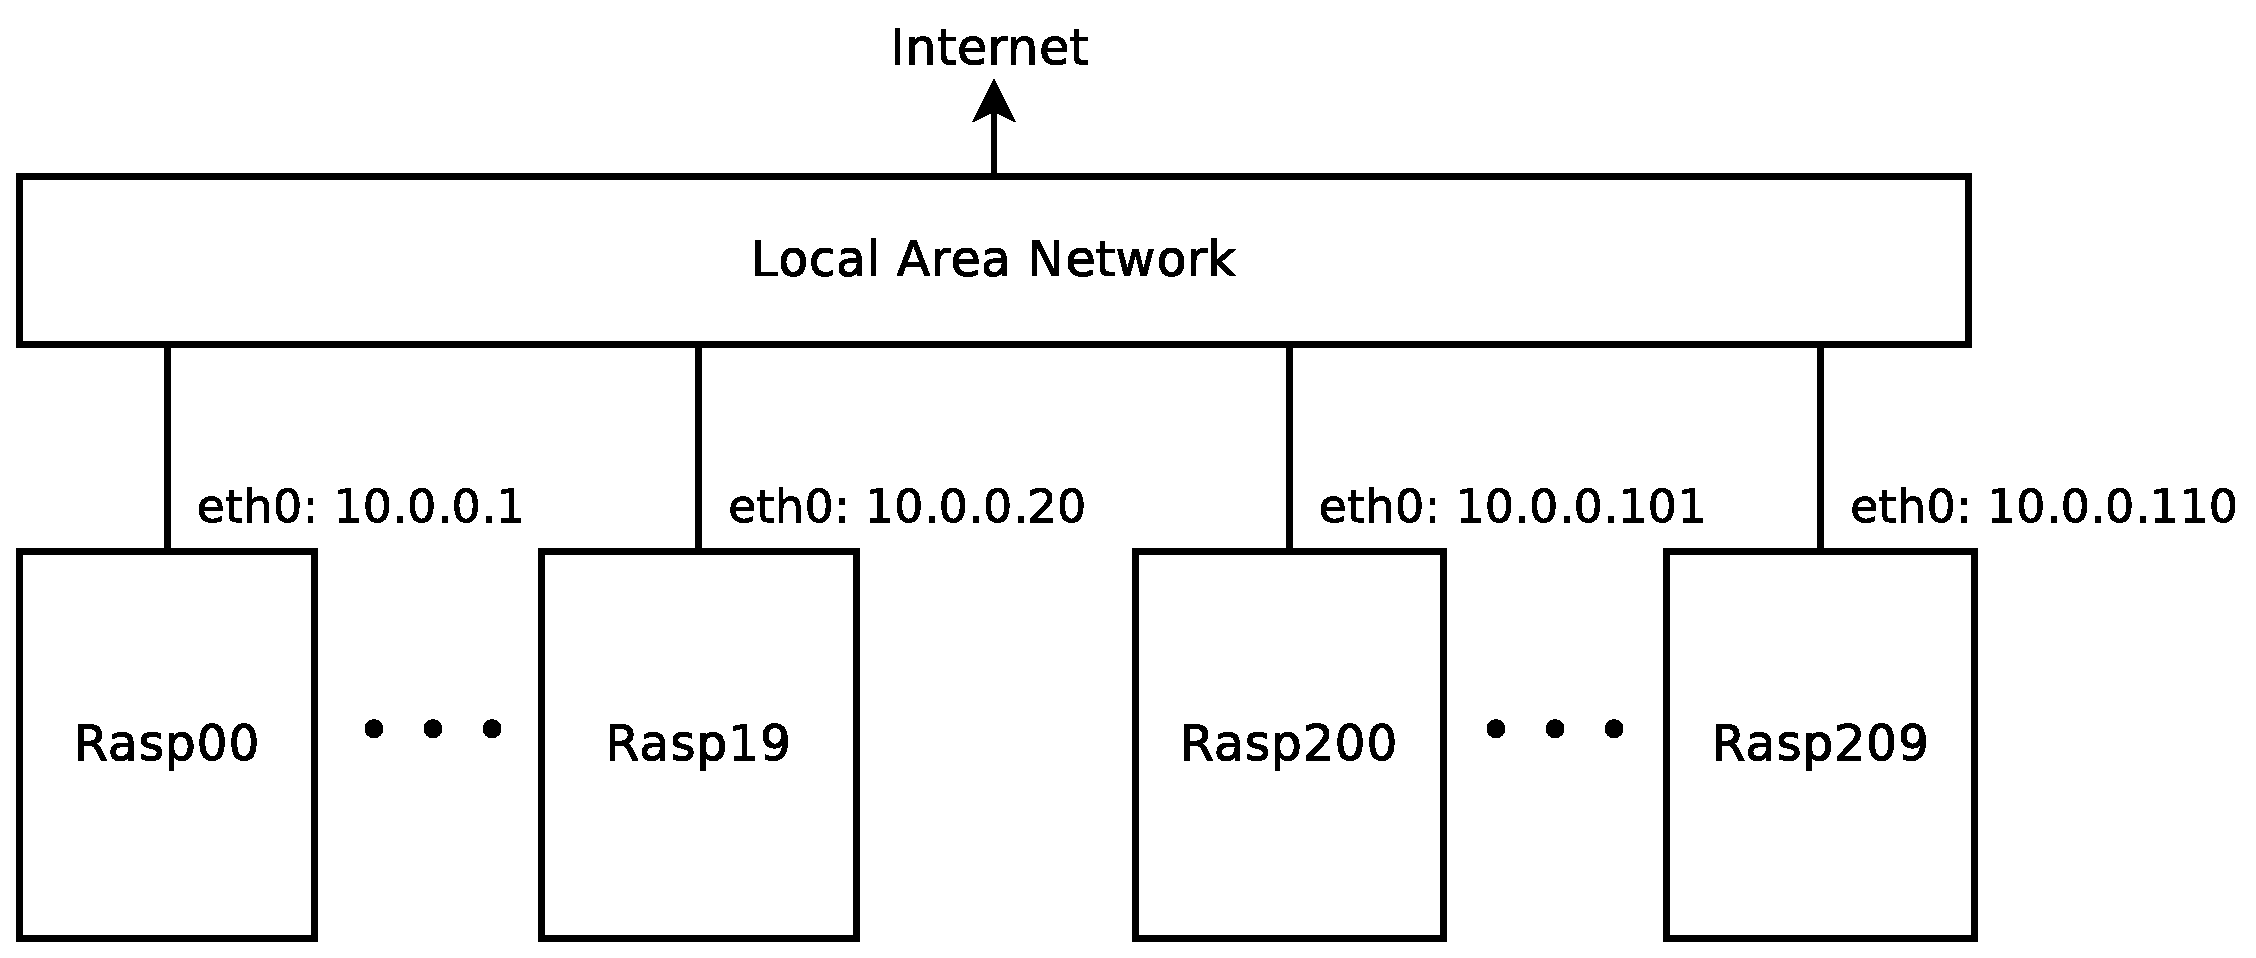
\includegraphics[width=0.6\textwidth]{images/testbed_setup.eps}
\caption{Testbed setup}
\label{fig:testbed_setup}
\end{figure}

\subsubsection{Installing Raspbian}

- 
- Download image (wget)
- Update/Modify image (chroot)
- Burn image
- Bang! linux is running
- 


We have installed the official Raspbian linux \ac{OS} on all the devices.



\subsection{Installation and Updating}
\subsection{Kodo cross-compilation: From your PC to the Raspberry Pi}

Besides the previous description (\textbf{Include compiling Kodo from the
RasPi from the scratch}), the testbed administrator can compile Kodo in its
personal workstation and transfer the generated binaries directly to
a path in the Raspberry Pi. To achieve this, we get a toolchain that
contains the binaries for the \texttt{raspberry-gxx49-arm-g++} compiler
for the Raspberry Pi. Therefore, we strongly recommend any testbed
administrator to do the following procedure. In what follows, we provide
the instructions considering that the NFS server uses the \texttt{\$HOME}
directory as the working directory. However, the administrator may choose
some other working directory of its preference if desired.

\begin{enumerate}

\item Download the Raspberry Pi toolchain for 64-bit Linux from: \\
\texttt{http://buildbot.steinwurf.dk/toolchains/linux/} to your
\texttt{\$HOME} directory. \\

\item Extract the downloaded file locally in the NFS server. After
this operation, there should be a new directory for the toolchain
in the server. \\

\item Add the \texttt{bin} folder of the toolchain to the \texttt{PATH}
Linux environment variable of the server. This will help the server OS
to recognize the location of the compiler command, which will be needed
later. To do so, edit the \texttt{\$HOME/.profile} to add in a newline:
\texttt{PATH="\$PATH:\$HOME/raspberry-gxx49-arm/bin"}. Save the
\texttt{\$HOME/.profile}. \\

\item Restart the server session in order for the changes made in the
previous step take effect. To verify this, open a new terminal and type:
\texttt{raspberry-gxx49-arm-g++ --version}. A correct binary installation
should return an output similar to:

\texttt{raspberry-gxx49-arm-g++ (crosstool-NG 1.21.0) 4.9.3 20150311 (prerelease)
Copyright (C) 2014 Free Software Foundation, Inc.
This is free software; see the source for copying conditions.  There is NO
warranty; not even for MERCHANTABILITY or FITNESS FOR A PARTICULAR PURPOSE.} \\

\item Clone the Kodo repository in the server by executing: \\
\texttt{git clone git://github.com/steinwurf/kodo.git} in \texttt{\$HOME}. \textbf{Change the repo to kodo-rlnc or kodo-cpp since just raw kodo is going to be depreceated soon} \\

\item Navigate to the repository and configure \texttt{waf} by typing:
\texttt{python config.py} and select the 16th ``make specification'' file
for the Raspberry Pi, e.g. option \texttt{[16]cxx\_raspberry\_gxx49\_arm}
presented by the file.

This command configures \texttt{waf} to use the proper compiler and its
required flags to generate the binaries for the Raspberry Pi. If the
configuration was correct, the output will indicate:
\texttt{'configure' finished successfully (X.XXXs)}, where \texttt{X.XXX}
is total time in seconds for configuring the project in the server. \\

\item Execute \texttt{python waf build}. If the build process was
successful, the generated binaries for the Raspberry Pi should be located
in \texttt{build/cxx\_raspberry\_gxx49\_arm} in the Kodo repository.
\textbf{Indicate how the binary files should look like}.

Once this procedure is made, the testbed administrator can relocate the
generated binary files to Raspberry Pi's through the network as desired
by using the \texttt{scp} command during the configuration step.


\end{enumerate}

\subsection{Kodo Builds for the Raspberry Pi, Platform Support and Documentation}

You can check the build status of Kodo, Fifi and other relevant projects through
their respective repository master branch on our buildbot page
\cite{steinwurf2016buildbot}. Our buildbot displays the status of the builds for
Raspbian 8 and GCC 4.9 for the ARM architecture which is the relevant one for the
Raspberry Pi. At the link, you can check build status and build statistics. Also,
documentation about Kodo basics with a tutorial is available at \cite{kododocs}.
